\documentclass[bsc,frontabs,twoside,singlespacing,parskip,deptreport]{infthesis}

\usepackage[round]{natbib}
\usepackage[hidelinks]{hyperref}

\usepackage{graphicx}

% Nice references including the words Figure, Section, etc
\renewcommand*{\sectionautorefname}{Section}
\renewcommand*{\subsectionautorefname}{Section}
\renewcommand*{\figureautorefname}{Figure}
\renewcommand*{\tableautorefname}{Table}
\newcommand{\algorithmautorefname}{Algorithm}
\renewcommand{\equationautorefname}{Eq.}

%
% TABLES
%

\usepackage{multirow} % multi-row and multi-column table cells
\usepackage{makecell} % line breaks inside cells with \thead{} and \makecell{}

% Globally setting the vertical padding in tables
\renewcommand{\arraystretch}{1.1}

% Spacing around lines in tables
\def\abovestrut#1{\rule[0in]{0in}{#1}\ignorespaces}
\def\belowstrut#1{\rule[-#1]{0in}{#1}\ignorespaces}
\def\abovespace{\abovestrut{0.17in}}
\def\aroundspace{\abovestrut{0.17in}\belowstrut{0.10in}}
\def\belowspace{\belowstrut{0.10in}}


\begin{document}

\title{\vspace{-5.0cm} \centering{\includeshield} \vspace{1cm} \\ Prosodic features in state-of-the-art \\spoken language identification}

\author{Sam Sucik}

\course{Master of Informatics}
\project{\vspace{3cm}{\bf MInf Project (Part 1) Report}}

\date{2019}

\abstract{
  TO-DO
}

\maketitle

% Add acknowledgements if necessary.
\section*{Acknowledgements}{
  Thanks to Paul Moore for productive collaboration while building the baseline system, to Steve Renals for his supervision and optimism, and to David Snyder for his advice.
}

\tableofcontents

%TO-DO: re-think and re-write
\chapter{Introduction}{
  \label{chap:Introduction}
  \section{Motivation}{
    LID is useful in ASR, in voice assistants, emergency call routing, etc.
    Traditionally, acoustic features are used (influence of ASR on LID and SID). Prosodic LID is much rarer, although results show that prosodic information can help identify language \citep{Lin_et_al_2005}, and that both LID and ASR can benefit from using acoustic \textit{and} prosodic features \citep{Martinez_et_al_2013,Ghahremani_et_al_2014}.
    Just last year, a novel architecture for LID utilising \textit{x-vectors} was proposed by \cite{Snyder_et_al_2018}, dramatically improving the state-of-the-art results. Although the authors find that using bottleneck features from an ASR DNN yields better results than using the standard acoustic MFCC features, even the ASR DNN was trained just using MFCCs. Thus the work ignores the potential of speech information other than that captured by MFCCs.
  }
  \section{Aims}{
    In this work, I aim to reproduce the state-of-the-art x-vector LID system and explore the use of prosodic features in addition to acoustic ones. Because the system uses a relatively novel architecture, in which a TDNN aggregates information across a speech segment, I also compare two types of acoustic features, one which has such aggregation over time encoded (SDC) and one that only contains information about single frames (vanilla MFCC).
  }
  \section{Contributions}{
    \begin{enumerate}
      \item {
        Adapted an existing x-vector speaker verification implementation (based on \cite{Snyder_et_al_2018b}) for language identification
      }
      \item {
        Explored the choice of classifiers and chose a different one than \cite{Snyder_et_al_2018}
      }
      \item {
        Prepared the Global Phone corpus for LID with the x-vector system, extending the original partitioning of the corpus into datasets and analysing invalid data
      }
      \item {
        Built and evaluated a baseline, end-to-end x-vector LID system using 19 languages of the Global Phone corpus
      }
      \item {
        Explored, set and tuned important hyperparameters of the system, mainly the number of training epochs of the x-vector TDNN
      }
      \item {
        Researched literature concerning the use of acoustic and prosodic features in language identification, speaker verification and ASR
      }
      \item {
        Designed, run and evaluated experiments comparing two types of acoustic features (MFCC and SDC) and two prosodic features (pitch, energy), and their combinations
      }
      \item {
        Built a system which has the potential to be open-sourced as part of the Kaldi ASR toolkit, to be used by a wider community
      }
    \end{enumerate}
  }
}

\chapter{Background}{
  \label{chap:Background}
  This chapter elaborates on the key concepts relevant to my work, as shown in this condensed description of the project: Exploring \textbf{spoken language identification} in the context of the recently proposed \textbf{x-vector} system (contrasted with the more established state-of-the-art \textbf{i-vector} approach, followed by the more novel \textbf{d-vector} systems), focusing on utilising \textbf{prosodic information} in addition to the standard \textbf{acoustic information}.

  \section{The task: spoken language recognition}{
    \label{sec:LID}
    Spoken language recognition means recognising the language of a speech segment. The task is similar to speaker recognition and, in the past, similar systems have been used for the two tasks. Importantly, recognition is typically realised as one of two different tasks: 
    \begin{itemize}
      \item {Identification (multi-class classification): answering the question "For a speech segment $X$, which one (from a number of supported targets) is its target (language or speaker) $T_x$?"}
      \item {Verification (binary classification): "Is $T_x$ the target (language or speaker) of the speech segment $X$?"}
    \end{itemize}
    Identification is more suitable for use cases with a small and stable set of possible targets -- such as the set of supported languages. There, computing the probability of $T_x$ being each of the target languages is feasible. Verification, on the other hand, is more suitable for cases where the set of possible targets less constrained -- such as the large and changing set of possible speakers in speaker verification systems. There, it is often infeasible to compute the probability distribution over all possible values of $T_x$; instead, the system typically focuses only on evaluating the probability of $T_x$ being the hypothesised speaker. Throughout this work, I focus on \textit{language identificaion} (LID) with a \textit{closed set} of target languages (i.e. not including the option to identify a speech segment's language  as unknown/other).
  }

  \section{Shallow utterance-level approach to LID: i-vectors}{
    \label{sec:i-vectors}
    This approach, with its numerous variations, has now been the state of the art for 8 years -- since first introduced by \cite{Dehak_et_al_2011} for speaker recognition and later applied by \cite{Martinez_et_al_2011} in language recognition.
    
    \begin{figure}[h!]
      \centering
      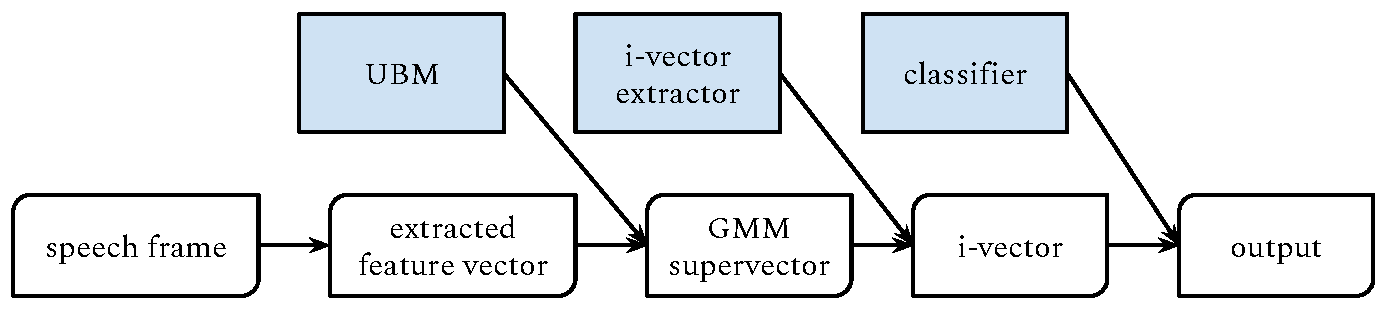
\includegraphics[width=14.5cm]{graphics/i-vectors}
      \vspace*{-1em}
      \caption{Language identification using a typical i-vector system.}
      \label{fig:i-vectors}
    \end{figure}

    The main components of a typical i-vector system, together with their use for prediction, are shown in \autoref{fig:i-vectors}. The universal background model (UBM) is a Gaussian mixture model (GMM) consisting of a large number (e.g. 2048) multivariate mixture components. The UBM is trained using the Expectation-Maximisation algorithm to model the observation space of frame-level feature vectors $\mathbf{x}$ computed from all training utterances (typically 39-dimensional vector using the MFCC features, see \autoref{sec:acoustic-feats}). Given the trained UBM, an utterance $X$ can be represented by a language- and channel-specific GMM supervector $M$ as:
    \begin{equation}
      \label{eq:supervector}
      M_X = m + Tw_X
    \end{equation}
    Here, $m$ is the language- and channel-independent GMM supervector of the UBM (consisting of the stacked means of all mixture components). $T$ is the \textit{total variability matrix} -- also called the i-vector extractor, and $w_x$ is the \textit{identity vector} (i-vector) of sample $X$. The total variability matrix $T$ is "a matrix of bases spanning the subspace covering the important [language and channel] variability in the supervector space" (\citeauthor[p.862]{Martinez_et_al_2011}). Effectively, $T$ projects between the high-dimensional GMM supervector space and the low-dimensional \textit{total variability subspace} (also called the \textit{i-vector space}). The i-vector $w_x$ is then a low-dimensional set of factors projecting the supervector onto the total variability subspace base vectors. The i-vector extractor $T$ is trained again using Expectation-Maximisation (for details see \citet[p. 100]{ivector_tutorial}). Without providing too much detail, I highlight the aspect that is most relevant to my work: training $T$ is based on calculating and further combining the 0\textsuperscript{th}, 1\textsuperscript{st} and 2\textsuperscript{nd} order statistics which are computed by \textit{summing over the frames} of an utterance.

    Once the i-vector extractor has been trained, any utterance can be represented by its i-vector. This enables training a relatively simple and fast classifier operating over the low-dimensional i-vectors. Different classifiers have been successfully used with the i-vector back end; for example, \citeauthor{Martinez_et_al_2011} initially tried using these, all achieving roughly equal performance:
    \begin{enumerate}
      \item {a linear generative model -- modelling the i-vectors of each language by a Gaussian, with a shared full covariance matrix across all language-modelling Gaussians}
      \item {a linear Support Vector Machine computing scores for all languages by doing binary classification in the one-versus-all fashion}
      \item {a two-class logistic regression also doing one-versus-all classification.}
    \end{enumerate}

    At test time, a sequence of feature vectors for utterance $X$ is projected using the UBM into the high-dimensional \textit{supervector space}, producing $M_X$. Then, $T$ is used to extract the utterance-level i-vector, which is processed by the classifier.

    Despite producing utterance-level scores, I describe the i-vector pipeline as shallow because it aggregates frame-level information over time very early (when projecting $X$ into the supervector space), effectively treating an utterance as a bag of frames and disregarding any temporal patterns spanning over multiple frames.
  }

  \section{Less shallow approach: d-vectors}{
    \label{sec:d-vectors}
    % in short: creating utterance-level representations by extracting frame-level information and averaging over frames
    % main difference compared to i-vectors: looking at sequences, i.e. taking each frame's surrounding context into account (this was done by both Variani and Tkachenko)
    % nothing changes about the classifiers, just a different way of producing vectors
    Introduced for speaker verification by \citet{Variani_et_al_2014} and later adapted and applied to language identification by \citet{dvectors_lid}, this approach uses neural networks to extract frame-level information, which is then aggregated across frames to produce utterance- or language-level vectors. Importantly, nothing changes about the final classification stage itself: It is the differences in producing the vector representations what makes i-vectors, d-vectors and x-vectors differ from each other.
    

    % context aggregation done using standard DNN but Tkachenko used TDNN, more familiar from ASR acoustic models and better suited for processing sequences (translation-invariant)
    The biggest change introduced in d-vector systems compared to i-vectors is the notion of frame-level processing while considering each frame's temporal context, i.e. the sequence of a few preceding and following frames. While \citeauthor{Variani_et_al_2014} achieve this by simply feeding the feature vectors of the neighbouring frames together with the frame of interest into a standard deep neural network, \citeauthor{dvectors_lid} use a more suited architecture commonly used for processing temporal sequences in automatic speech recognition: the \textit{time-delay neural network} (TDNN).

    % describing TDNN: like 1D CNN. often made sparse. aggregates information along the time axis
    % TO-DO: Advantages of TDNN over a fully connected DNN?
    % TO-DO: Mention where was TDNN first introduced?
    \begin{figure}[h!]
      \centering
      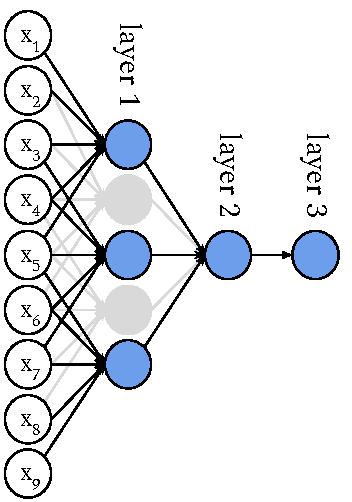
\includegraphics[height=6cm]{graphics/tdnn-generic}
      \caption{Example of a time-delay neural network.}
      \label{fig:tdnn-generic}
    \end{figure}
    A TDNN works like a convolutional neural network (CNN) with 1-dimensional convolutions: only along the time axis, as opposed to the more common 2-dimensional convolutions in image CNNs. \autoref{fig:tdnn-generic} shows a TDNN with three layers which processes information over 9-frame contexts. Note that each blue circle from any layer corresponds to the layer itself (a collection of neurons, i.e. \textit{convolutional kernels}), and all blue circles drawn above each other as corresponding to a particular layer are in fact just one circle -- the layer itself -- sliding over multiple inputs. For example, the convolutional kernels from layer 1 are first applied to feature vectors $\mathbf{x_1}$-$\mathbf{x_5}$, then to vectors $\mathbf{x_3}$-$\mathbf{x_7}$ and then to $\mathbf{x_5}$-$\mathbf{x_9}$. Notice how the network is made more sparse by using \textit{subsampling}, i.e. not using the connections drawn in light grey. A concise and commonly used description of the sketched architecture is shown in \autoref{tab:tdnn-generic} (notice the difference between the interval and set notation); "layer context" meant relative to the preceding layer.
    \begin{table}[h!tb]
      \centering
      \begin{sc}
        \begin{tabular}{l|cc}
                      & Layer context      & Total context \\
          \hline
          layer 1     & $[t-2,\ t+2]$      & 5 \\
          layer 2     & $\{t-2,\ t,\ t+2\}$& 9 \\
          layer 3     & $\{t\}$            & 9 \\
        \end{tabular}
      \end{sc}
      \caption{Example of architecture description of a TDNN (corresponds to \autoref{fig:tdnn-generic}).}
      \label{tab:tdnn-generic}
    \end{table}

    % trained by doing frame-level classification. then the softmax layer ignored and getting activations from the last hidden layer. embeddings! also, GMM supervectors are some kind of embeddings as well ;-)
    In a d-vector system, a TDNN is trained to do direct frame-wise language identification; for this purpose, an additional softmax layer can be added to produce classification outputs. Often, between the convolutional layers and the output layer the architecture contains a few fully connected layers. After training, the classification layer is disregarded and a frame is instead represented by the activation values from the last hidden layer. The TDNN thus serves as a feature extractor, and the representations produced are referred to as \textit{embeddings}.
    % averaging to get utterance-level or language-level vectors.  which after extracting information from frames with contexts, average
    A d-vector representing an entire utterance is then simply the average of the embeddings of all frames from the given utterance.
    
    % even though information is simply averaged across frames, d-vectors made a step beyond bag of frames: temporal features are being extracted, in the case of Tkachenko +-10 (21-frame window), Variani did -30 +10 (41-frame window)
    Despite the naive averaging, utterances are no longer treated merely as bags of frames because each embeddings contains features extracted over short temporal window: 21-frame windows in the case of \citeauthor{dvectors_lid} and 41-frame windows used by \citeauthor{Variani_et_al_2014}, making d-vectors less shallow than i-vectors.
  }

  % TO-DO: justify the use of 'deep'
  \section{Deep utterance-level approach: x-vectors}{
    \label{sec:x-vectors}
    % natural extension to d-vectors: computing not just average but also standard deviation.
    The x-vector approach, introduced last year by the John Hopkins University team first for speaker verification \citep{Snyder_et_al_2018b} and subsequently for language identification \citep{Snyder_et_al_2018}, can be viewed as an extension to d-vectors, producing utterance-level embeddings even for variable-length speech segments. The architecture consists of (see also \autoref{fig:x-vectors-hl}):
    \begin{enumerate}
      \item {the context-aggregating TDNN layers operating at frame level (with the final context window of $\pm$7 frames),}
      \item {a \textit{statistics pooling layer} which computes the mean and the standard deviation over all frames, effectively changing a variable-length sequence of frame-level activations into a fix-length vector, and}
      \item {an utterance-level part consisting of 2 fully connected bottleneck layers which extract more sophisticated features and compress the information into a lower-dimensional space, and an additional softmax output layer.}
    \end{enumerate}
    
    \begin{figure}[h!]
      \centering
      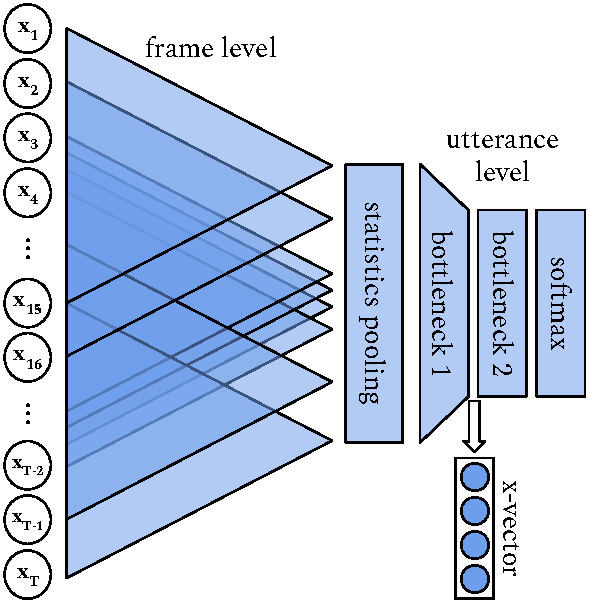
\includegraphics[height=8cm]{graphics/x-vectors-hl}
      \caption{A high-level sketch of the x-vector TDNN from \citeauthor{Snyder_et_al_2018}.}
      \label{fig:x-vectors-hl}
    \end{figure}
    % bottleneck layers to extract _small_ enbeddings
    % biggest difference: TDNN trained to do utterance-level classification (likely to improve the quality of embeddings)
    After the TDNN has been trained, embeddings extracted as the activations of the first bottleneck layer -- named x-vectors -- are then utterance-level representations and can be used directly as input for a final classifier. The biggest difference compared to the d-vector neural networks discussed in \autoref{sec:d-vectors} is that the x-vector TDNN is trained to do not frame-level, but utterance-level classification. The utterance-level statistics (mean and standard deviation) are computed \textit{as part of the network} and are further processed by the additional fully connected layers with non-linear activation functions. These bottleneck layers also make it possible to preserve a higher number of useful features after the statistics-pooling layer: By enabling the last frame-level layer to inflate the representations to 1500-D. The bottleneck layers then learn a transform back to the 512-dimensional space (high-dimensional vectors would be inconvenient for the final classifier) while extracting from the aggregated statistics the features most useful for utterance-level classification (not just for frame-level decisions).

    \begin{table}[h!tb]
      \centering
      \begin{sc}
        \begin{tabular}{cl|ccc}
                      && Layer context      & \thead{Total \\ context} & Number of units \\
          \hline
          \multirow{5}{*}{\rotatebox[origin=c]{90}{frame level\ }}
          &layer 1     & $[t-2,\ t+2]$      & 5             & 512 \\
          &layer 2     & $\{t-2,\ t,\ t+2\}$& 9             & 512 \\
          &layer 3     & $\{t-3,\ t,\ t+3\}$& 15            & 512 \\
          &layer 4     & $\{t\}$            & 15            & 512 \\
          \belowspace
          &layer 5     & $\{t\}$            & 15            & 1500 \\
          \hline
          \multicolumn{2}{c|}{\makecell{statistics pooling \\ layer}} 
                       & $[1,T]$            & utterance     & \makecell{3000-dimensional\\ output} \\
          \hline
          \abovespace
          \multirow{3}{*}{\rotatebox[origin=c]{90}{\shortstack[l]{utter.\\level}}}
          & bottleneck 1& N/A               & utterance     & 512 \\
          & bottleneck 2& N/A               & utterance     & 512 \\
          & softmax     & N/A               & utterance     & \makecell{L-dimensional \\ output} \\
        \end{tabular}
      \end{sc}
      \caption{Description of the x-vector TDNN from \citeauthor{Snyder_et_al_2018} and used in this work. $T$~is the number of frames in a given utterance. Table adapted from \citet[p. 106]{Snyder_et_al_2018}.}
      \label{tab:x-vectors}
    \end{table}

    % trained architecture can be used directly as an end-to-end LID classifier, but found to perform better when x-vectors are extracted and fed into separate classifier. also, adding new languages is possible with classifier and has been shown to perform well even when the TDNN didn't see the language during training
    Because of being an utterance-level classifier, the x-vector TDNN can be used directly as an end-to-end system, although \citeauthor{Snyder_et_al_2018} found that extracting x-vectors and training a separate classifier to classify them yielded lightly better results. Perhaps an even stronger argument in favour of the two-stage process is that, by using an external light-weight classifier, one can easily change the set of supported languages without having to expensively re-train the TDNN. \citeauthor{Snyder_et_al_2018} showed that simply re-training the classifier is enough to gain very good results for languages the TDNN has not observed during training (although the results are indeed worse than those for observed languages).

    % outperforming various optimized variations of i-vectors
    % TO-DO: Define somewhere the metric used to compare the systems and provide concrete numbers?
    The x-vector system consistently beat several state-of-the-art i-vector architectures, which is a particularly interesting finding because i-vector systems have for long been dominant despite the nowadays so "fashionable" and successful deep learning approaches. Even so, the 2-stage x-vector system using a simple classifier still dominates the end-to-end neural network alternative.
  }

  \section{Features used in language identification}{
    \label{sec:features}
    % ASR being the main speech processing area and the powerhorse of research; to an extent, LID systems are motivated by ASR systems which need to know the language first
    Historically, automatic speech recognition (ASR) has been the most important area of speech processing and it has driven forward other areas including language and speaker recognition. In particular, LID systems still exist mostly as part of ASR systems where the language of speech needs to be identified before attempting to transcribe the speech.
    % Hence, most feature engineering has been done with the aim of extracting information useful for ASR -- the speaker- and language-independent information on the phones produced by the vocal tract. These are called acoustic features.
    Hence, data preprocessing and input feature types for LID systems often come from the ASR area. In particular, the feature extraction processes follow the ASR objectives: To extract the language- and speaker-\textit{independent} information important for discriminating between different phonemes produced by a speaker's vocal tract. The feature types devised for this aim are termed \textit{acoustic features}.
    % Acoustic feats can also be described in terms of the information they disregard or do not explicitly capture: information which is language- and speaker-specific -- intonation, stress, pitch range, tone, and others, collectively referred to as prosodic information.
    However, these features can also be characterised by the information they disregard or at least to not capture explicitly: the language- and/or speaker-\textit{dependent} information: intonation, stress, pitch range, tone, and others, collectively referred to as \textit{prosodic information}.
    
    % Since this work focuses on using prosodic information to improve LID, it is useful to understand both acoustic and prosodic features, how they differ and how prosody can be utilised by systems that process frame sequences rather than individual frames.
    As this work focuses on exploiting prosodic information to improve LID, it is desirable to understand both acoustic and prosodic features: how they differ, why is prosody useful and how can prosodic information be modelled in systems that process frame sequences rather than isolated speech frames.

    % TO-DO: Mention that acoustic are more accent-independent while prosodic may be misleading e.g. for non-native speakers.
    
    \subsection{Acoustic features}{
      \label{sec:acoustic-feats}
      % Most common acoustic feats: MFCCs. Their aim is literally to describe the shape of the vocal tract (which maps to the shape of the spectral envelope, which maps to the phone produced).
      The most commonly used acoustic feature type are the Mel-frequency cepstral coefficients (MFCCs). These are coefficients that aim to characterise the shape of the vocal tract, which corresponds to characterising the spectral envelope of produced sounds or, in a way, to the actual phones produced. Without providing too much technical detail, I remind the reader of the main steps in computing MFCCs in \autoref{fig:mfcc} (for details, see for example Chapter 10 of \citet{Holmes_and_Holmes}).
      % Image of MFCC pipeline with high-level descriptions of single steps.
      % - windowing: extracting short temporal frames from the waveform
      % - extracting enery level (loudness) from each frame
      % - discrete fourier transform: extracting spectral information from a single frame (transform from time domain into frequency domain)
      % - mel filterbank: quantifying the energy levels present in discrete, overlapping frequency bands (spaced unevenly to reflect the human perceptual scale), smoothing out pitch information
      % - logarithm: accounting for human non-linear perception of loudness
      % - inverse DFT: extracting coefficients characterising the shape of the spectral envelope
      \begin{figure}[h!]
        \centering
        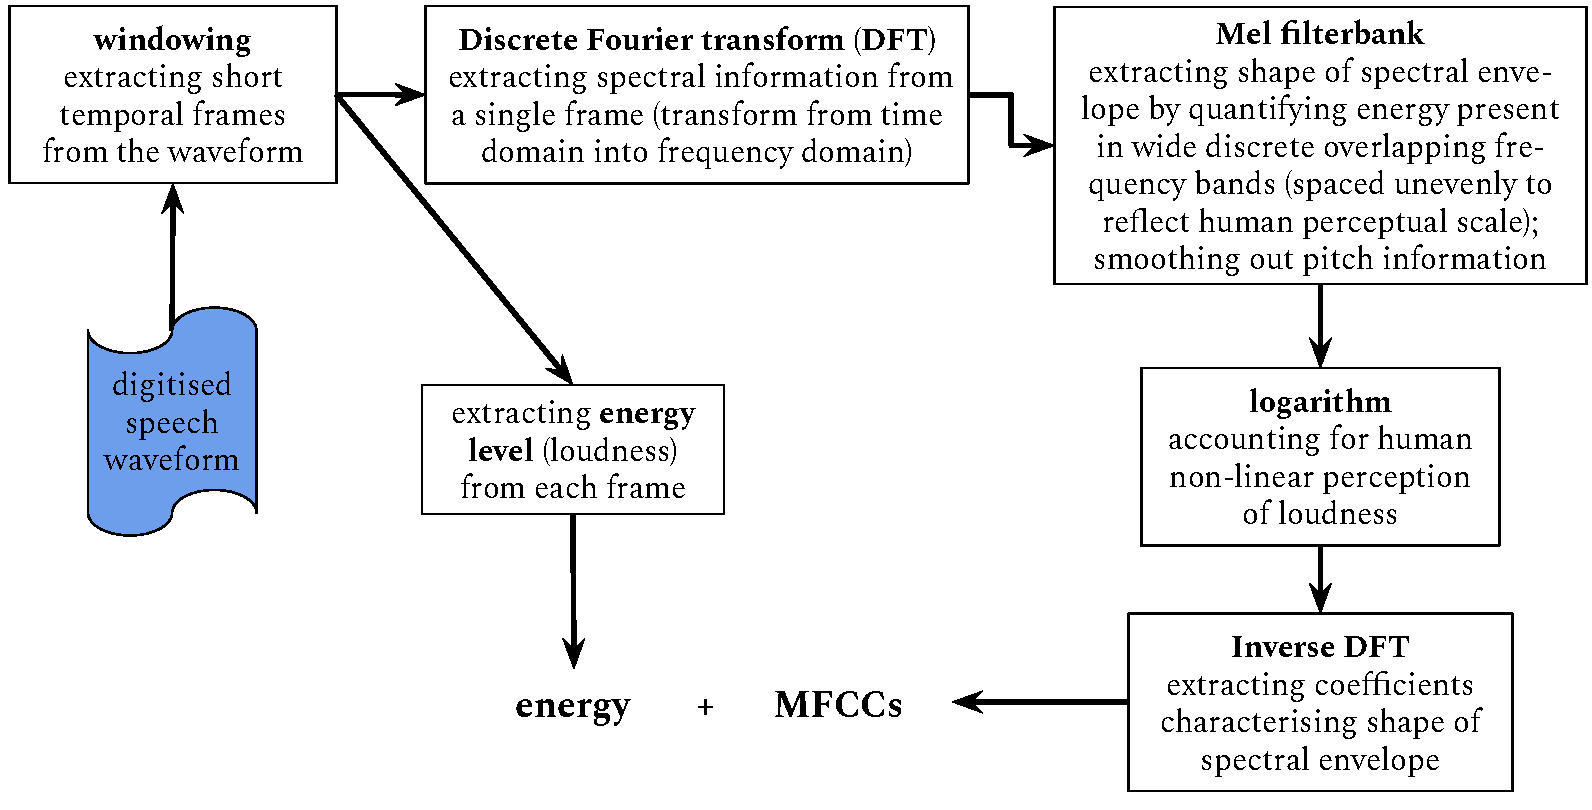
\includegraphics[width=\textwidth]{graphics/mfcc}
        \vspace*{-1em}
        \caption{Main steps in computing the MFCC features including energy. Adapted from \citet[p. 10]{ASR_L2}.}
        \label{fig:mfcc}
      \end{figure}
      % Note that recently, mel filterbanks have been used as well, because neural networks can deal well with correlated features, and doing one less feature processing step is attractive (with each step, some information is lost).

      % To explicitly capture local temporal trends, delta and delta-delta terms are often computed and added to MFCCs or mel filterbanks
      To capture local temporal trends going beyond the single frame level, computed features such as MFCCs are often augmented with frame-specific \textit{dynamic} features -- \textit{delta cepstra} (also just \textit{deltas} or $\Delta$) and double deltas ($\Delta\Delta$). These are simple approximations of the first and second derivatives of the original acoustic feature, and are computed for frame $t$ like this ($\mathbf{x}_t$ is the MFCC feature vector):
      \begin{equation}
        \label{eq:dynamic-feats}
        \Delta(t) = \mathbf{x}_{t+1} - \mathbf{x}_{t-1},\ \ \ \ \Delta\Delta(t) = \Delta(t+1) - \Delta(t-1)
      \end{equation}
      using the context of~$\pm$2~frames. Such dynamic features are justified especially in systems which apply the bag-of-frames approach, not extracting temporal trends (such as the standard i-vector architectures).

      % To capture temporal trends over longer contexts, MFCCs are often turned into SDCs.
      For modelling even longer-range trends specifically in the LID task, \citet{Torres-Carrasquillo_et_al_2002} used an extension of simple deltas called the \textit{shifted delta cepstra} (SDC) features -- essentially, deltas computed at multiple points and concatenated with the original MFCC vector as previously. SDCs can be configured by setting their 4 parameters: $N$, $d$, $p$, $k$ corresponding to a $N$-$d$-$p$-$k$, a typical one being 7-1-3-7. $N$ refers to the number of cepstral coefficients taken into account (not necessarily the full MFCC vector), $p$ denotes the distance between consecutive points at which deltas are computed, $d$ determines the size of the window for computing deltas ($d=1$ corresponds to \autoref{eq:dynamic-feats}) and $k$ is the number of points at which to compute deltas. The SDCs added to the original MFCC vector are then of the form:
      \begin{equation}
        \label{eq:sdc-feats}
        \Delta_{SDC}(t+ip) = \mathbf{x}_{t+ip+d} - \mathbf{x}_{t+ip-d} \quad\quad \forall i \in \{0, ..., k-1\}
      \end{equation}
      % SDC used by \cite{Ferrer_et_al_2016} and \cite{Sarma_et_al_2018} (7D MFCC + 7-1-3-7 SDCs = 56D) and by \cite{Torres-Carrasquillo_et_al_2002} (10-1-3-3)
      As with standard deltas, capturing long-range trends with SDCs can certainly be beneficial for i-vector systems. \cite{Ferrer_et_al_2016} used an i-vector system with SDC features as the state-of-the-art baseline system for their novel experiments. Additionally -- following the successful application of SDCs by \citeauthor{Torres-Carrasquillo_et_al_2002} in a pre-i-vector system, \cite{Sarma_et_al_2018} report slightly better results with SDCs compared to using high-resolution MFCCs when training an i-vector architecture with a deep neural network UBM. Still, the usefulness of SDCs is not so clear in architectures inherently able to extract temporal trends.

      % Advantage of acoustic features for LID: where LID is part of ASR, acoustic feats are available anyway, hence there's no need to compute different feats just for the LID part.
      Compared to the prosodic features described next, the discussed classic acoustic features have one clear advantage where the LID system is part of a bigger ASR pipelines: The two systems can share the same feature vectors without the need to compute additional features solely for the purpose of language identification.

      % MFCCs also used inderectly to train ASR DNNs which then provide bottle-neck features which give very promising results in both LID and SID
    }

    % LEL2D lecture on tone: https://www.learn.ed.ac.uk/bbcswebdav/pid-2255587-dt-content-rid-4289141_1/courses/LASC080202016-7SV1SEM2/week05.02.html
      % A language with tone is one in which an indication of pitch enters into the lexical realization of at least some morphemes (Hyman 2006) Hyman, Larry M. 2006. Word-prosodic typology. Phonology 23(2). 225–257.
      % A language is a ‘tone language’ if the pitch of the word can change the meaning of the word. Not just its nuances, but its core meaning. (Yip 2002) Yip, Moira. 2002. Tone. Cambridge: Cambridge University Press.
    \subsection{Prosodic features}{
      \label{sec:prosodic-feats}
      % OLD MATERIAL TO BE RE-USED
        % compared to well-established acoustic feats, there is no good definition of prosodic feats and they are not commonly used
        % for the purposes of this work, I narrow down the prosodic variables to four: intonation+tone, stress and rhythm. TO-DO: these should be the main ones, cite some paper?
        
        % both intonation and tone are perceived qualities, typically associated with the variation of the physical quality called pitch, i.e. the fundamental frequency of vibration of the vocal folds (also denoted as F_0). 
        % while the term 'tone' is used where pitch variation is contrastive (i.e. changes to it discriminate between different words) in the so-called tonal languages (such as Chinese, Vietnamese, Thai), intonation denotes the non-contrastive pitch variation mostly associated with speaker's emotions, dialect, social background, speaking style, and other factors (see, for example, this study by \citet{Grabe_2004} on the intonation differences across British English dialects).
        % note: some recent results show what other physical variables can influence perceived intonation, but these are disregarded for now. TO-DO: find those works?
        % \citet{Lin_et_al_2005} do LID just from the segmented pitch contour, each short pitch segment (around 100-200ms) parametrised by a few Legendre polynomials -- not too much success
        % \citet{Metze_et_al_2013} show improvements in ASR on tonal (and partly on non-tonal) languages when including F0 variation feats.
        % \citet{Song_et_al_2013} achieve LID improvements when using bottleneck features trained on MFCC+pitch vectors
        % One disadvantage of pitch contours: F0 is undefined for unvoiced sounds, hence the computed pitch contour is not continuous.
        % \cite{Ghahremani_et_al_2014} show ASR improvements with a pitch-tracking algorithm that calculates pitch even for unvoiced frames, creating continuous pitch contours. to the best of my knowledge, this feature type hasn't yet beet applied in an LID task.

        % stress (also termed accent) is an unstable term, generally referring to relative emphasis on certain syllables or words and realised as a variation in loudness (dynamic accent), pitch (pitch accent) or length (quantitative accent).
        % ASR models dynamic and quantitative accent implicitly under certain conditions when using acoustic feats. but I isolate 

        % in this work, I contrain myself to using two feature types for modelling prosody: 
        % - continuous pitch contours extracted using the KaldiPitch algorithm (introduced by \cite{Ghahremani_et_al_2014}) - I refer to this as the pitch feature
        % - raw energy capturing the loudness of speech and modelling dynamic stress (at both word and sentence level)
      % END OF OLD MATERIAL

      % NEW MATERIAL
      % 1. short intro into prosody (cite WALS where appropriate)
      % Prosody stands for information other than that about the produced phonemes. Standard elements: intonation/tone, stress, rhythm. As shown below, each of these can be used to differentiate between languages.
      Prosody is about information other than that directly describing the produced phones; the standard elements of prosody are: intonation/tone, stress and rhythm \citep{Prieto_et_al_2018}. As discussed below, importantly, each of these elements can be used to differentiate between languages.
      \begin{itemize}
        % - intonation and tone are perceived qualities, typically associated with the variation of the physical quality called pitch, i.e. the fundamental frequency of vibration of the vocal folds (F0). while the term 'tone' is used where pitch variation is contrastive (i.e. changes to it discriminate between different words) in the so-called tonal languages (such as Chinese, Vietnamese, Thai), intonation denotes the non-contrastive pitch variation mostly associated with speaker's emotions, dialect, social background, speaking style, and other factors (see, for example, this study by \citet{Grabe_2004} on the intonation differences across British English dialects).
        \item {\textit{Intonation} and \textit{tone} are perceived qualities typically associated with the variation of the physical quality called pitch, i.e. the fundamental frequency of vibration of the vocal folds ($F_0$). The term 'tone' is used where pitch variation is contrastive (i.e. changes to it discriminate between different words): in the so-called \textit{tonal languages}, such as Chinese, Vietnamese and Thai. In each of these languages, a small 'alphabet' of distinct tone levels or tone contours can be observed as it conveys meaning. Intonation, on the other hand, denotes the non-contrastive pitch variation mostly associated with the speaker's emotions, language, dialect, social background, speaking style, and other factors (see, for example, the study by \citet{Grabe_2004} on the intonational differences between different British English dialects).}
        % - stress (also termed accent) is an unstable term, generally referring to relative emphasis on certain syllables or words and realised as a variation in loudness (dynamic accent), pitch (pitch accent) or vowel length (quantitative accent). Specific lexical (syllable-level) stress patterns or rules are often characteristic of a language, e.g. the position of stress is fixed to different positions within word in Czech and Polish (fixed stress), or describable by a set of rules in Arabic (rule-based stress, this needs citation).
        \item {\textit{Stress} (also termed \textit{accent}), despite being a somewhat ambiguous term, generally refers to the relative emphasis on certain syllables within a words or words within a sentence, realised as a variation in loudness (\textit{dynamic accent}), pitch (\textit{pitch accent}) or vowel length (\textit{quantitative accent}). Specific \textit{lexical} (intra-word, i.e syllable-level) stress patterns or rules are often characteristic of a language. For instance, the within-word location of stress is fixed but different for Czech and Polish (\textit{fixed stress}, see \citet{WALS_14}), or describable by a set of rules in Arabic (\textit{rule-based stress}, see \citet{WALS_15}).}
        % - rhythm typically refers to syllable lengths, with the theory of isochrony categorising languages into three types based on their rhythm: syllable-timed, e.g. french or turkish (all syllables have roughly equal durations), mora-timed, e.g. slovak or japanese (all moras have equal durations) and stress-timed languages, e.g. german, arabic (intervals between stressed syllables are of equal durations).
        \item {\textit{Rhythm} refers to regularity in sub-word unit lengths, with the most recognised theory of \textit{isochrony} categorising languages into three types based on their rhythm: \textit{syllable-timed} where all syllables have roughly equal durations (e.g. French or Turkish), \textit{mora-timed} where all moras\footnote{Mora is a basic timing unit; a long syllable having two moras and a short syllable having one mora. See \citet[p. 312]{Crystal_2008} for a broader definition and discussion.} have equal durations (e.g. Slovak or Japanese), and \textit{stress-timed} languages, e.g. German and Arabic (here, the intervals between stressed syllables are of equal durations).}
      \end{itemize}

      % isochrony details
        % syllable-timed: french, spanish, mandarin, turkish
        % mora-timed: japanese, slovak, tamil (https://www.sissa.it/cns/Articles/TBC_048.pdf)
        % stress-timed: thai, german, russian, swedish, portuguese (EU), arabic
        % bulgarian (http://www.personal.reading.ac.uk/~llsroach/phon2/sdjipa.htm), polish (https://www.sissa.it/cns/Articles/TBC_048.pdf): between stress-timed and syllable-timed

      % TO-DO: comment on temporal ranges? 15 frames cover variation across maybe 1-2 syllables. duration of syllable: some 100-200 ms (https://core.ac.uk/download/pdf/84560.pdf)
      % 2. what prosodic aspects acoustic features can capture: rhythm, quantitative stress
      % some of the mentioned prosodic aspects can in fact be captured even when using acoustic features like MFCCs. because prosody surfaces as temporal variation, systems which extract features from frame sequences (such as x-vectors) have the potential to capture it (unlike i-vector systems which apply the bag-of-frames approach). MFCCs can contain information about loudness (in the form of the energy-based C0 cepstral coefficient), which enables capturing dynamic stress. even without using C0, quantitative accent should be possible to capture using acoustic features. regarding rhythm, the temporal trends should be possible to capture for syllable-timed and mora-timed languages, but not necessarily for stress-timed languages (if C0 is not used or if the stress patterns rely heavily on pitch accent which cannot be captured using acoustic features). considering the prosodic aspects that acoustic features alone could theoretically capture, the most important prosodic feature that can be added to the input is pitch: to enable modelling pitch accent, tone, and language-specific intonation.
      Before turning to bespoke alternative features for modelling prosody, it should be noted that some prosodic aspects can be captured by acoustic features like MFCCs. Because prosody surfaces as temporal variation, systems which extract information from frame sequences (such as TDNN-based systems) have the potential to capture it. MFCCs can be (and often are) used together with energy (see \autoref{fig:mfcc}), which enables capturing dynamic accent. Even without using energy as part of MFCCs, the quantitative accent should be possible to capture because durations of vowels are preserved as a result of windowing extracting the frames at evenly spaced points of a speech waveform. Regarding rhythm, the duration regularity (isochrony) should be possible to capture for syllable-timed and mora-timed languages because syllable boundaries occur at phoneme boundaries, which are captured by acoustic features. For stress-timed languages, however, the units with equal durations are marked by stressed syllables, meaning that this regularity may not be fully captured -- in particular if an energy measure is not included in MFCCs, or if the stress is realised as a variation in pitch rather than in loudness. Considering the prosodic aspects that acoustic features alone \textit{could} theoretically capture, I conclude that the most important prosodic feature that can be deemed complementary to acoustic features and added to the input is pitch: to enable modelling pitch accent, tone, and language-specific intonation.


      % 3. what prosodic aspects have been modelled explicitly: intonation/tone/pitch accent (pitch contours)
      % perhaps unsurprisingly, extracting information from pitch for LID has been explored in the past -- although the number of studies very small compared to those using conventional acoustic features. long before i-vectors, \citet{Lin_et_al_2005} attempted LID just from the pitch contour segmented into syllable-like units (around 100-200ms), contour segments parametrised by a few Legendre polynomials. later, \citet{Metze_et_al_2013} show improvements in ASR on tonal (and partly on non-tonal) languages when augmenting MFCCs with F0 variation features. One disadvantage of pitch contours: F0 is not present for unvoiced sounds, hence a pitch contour computed from F0 is not continuous. this issue was addressed by \cite{Ghahremani_et_al_2014} who developed a pitch-tracking algorithm that approximates the pitch contour even for unvoiced frames, making it continuous. they report improved ASR performance mainly on tonal languages. to the best of my knowledge, this feature type hasn't yet beet applied in an LID task.
      Perhaps unsurprisingly, extracting information from pitch for LID has been explored in the past -- although the number of studies is very small compared to those using the conventional acoustic features. Long before i-vectors, \citet{Lin_et_al_2005} attempted to do language identification solely from the pitch contour. This was segmented into syllable-like units (around 100-200ms), each contour segment subsequently represented as the first few coefficients of its approximation by Legendre polynomials. Even though the results were far from those achieved by today's systems, it was demonstrated that LID can be done on pitch information alone. Later, \citet{Metze_et_al_2013} showed improvements in ASR on tonal (and partly on non-tonal) languages when augmenting MFCCs with custom-designed $F_0$ variation features. Nevertheless, one disadvantage of using pitch persisted: The fact that $F_0$ is typically considered to be only present in voiced sounds and undefined for unvoiced ones -- making a pitch contour based on $F_0$ discontinuous. This inconvenience has been recently addressed by \cite{Ghahremani_et_al_2014} who developed a pitch-tracking algorithm that approximates pitch values even for unvoiced regions and produces a continuous pitch contour. Adding this feature to MFCCs, the authors report improved ASR performance mainly on tonal languages. To the best of my knowledge, this feature type has not yet been used for language identification.


      % 4. what features I use to explicitly model prosodic aspects: KaldiPitch, raw energy
      % In this work I explore two feature types that explicitly help to capture prosodic information: energy and pitch. I refer to these as the prosodic features.
      In this work, I explore two feature types that explicitly help to capture prosodic information: \textit{energy} and \textit{pitch}. I refer to these as the prosodic features.
      \begin{itemize}
        % By energy I mean the logarithm of the raw energy extracted in the MFCC pipeline right after pre-emphasis and windowing. To isolate the effects of using this prosodic feature, I do not include it in any of the acoustic features used in this work.
        \item {By energy I mean the logarithm\footnote{The use of logarithm is given solely by the Kaldi toolkit I use for feature extraction, although it is by no means an arbitrary design decision: Human perception of loudness is non-linear and logarithm is used also in the standard MFCC computation pipeline (see \autoref{fig:mfcc}).} of the raw energy extracted in the MFCC pipeline right after windowing (as shown in \autoref{fig:mfcc}). To isolate the effects of using this prosodic feature, I do not include it in any of the acoustic features used in this work. However, I do not exclude the 0\textsuperscript{th} cepstral coefficient from MFCCs, even though it bears some loudness-related information; more specifically, it can be considered as "a collection of average energies of each frequency bands in the signal that is being analyzed" \citep{Zheng_and_Zhang_2000}.}
        % By pitch I mean the continuous pitch extracted using the algorithm presented by \citeauthor{Ghahremani_et_al_2014}.
        \item {By pitch I mean the continuous pitch (and features derived from it) extracted using the Kaldi pitch algorithm presented by \citeauthor{Ghahremani_et_al_2014}. Because this feature type is not well known, I elaborate on it in the next section.}
      \end{itemize}
    }
    \subsection{The continuous Kaldi pitch as a prosodic feature}{
      \label{sec:kaldi-pitch}
      Even though the original paper \citep{Ghahremani_et_al_2014} contains a detailed description of the Kaldi pitch algorithm (along with a working implementation as part of the Kaldi ASR toolkit), I provide an additional, more holistic view to give the reader an intuitive understanding of the algorithm and the features it produces (see \autoref{fig:kaldi-pitch}).
      \begin{figure}[h!]
        \centering
        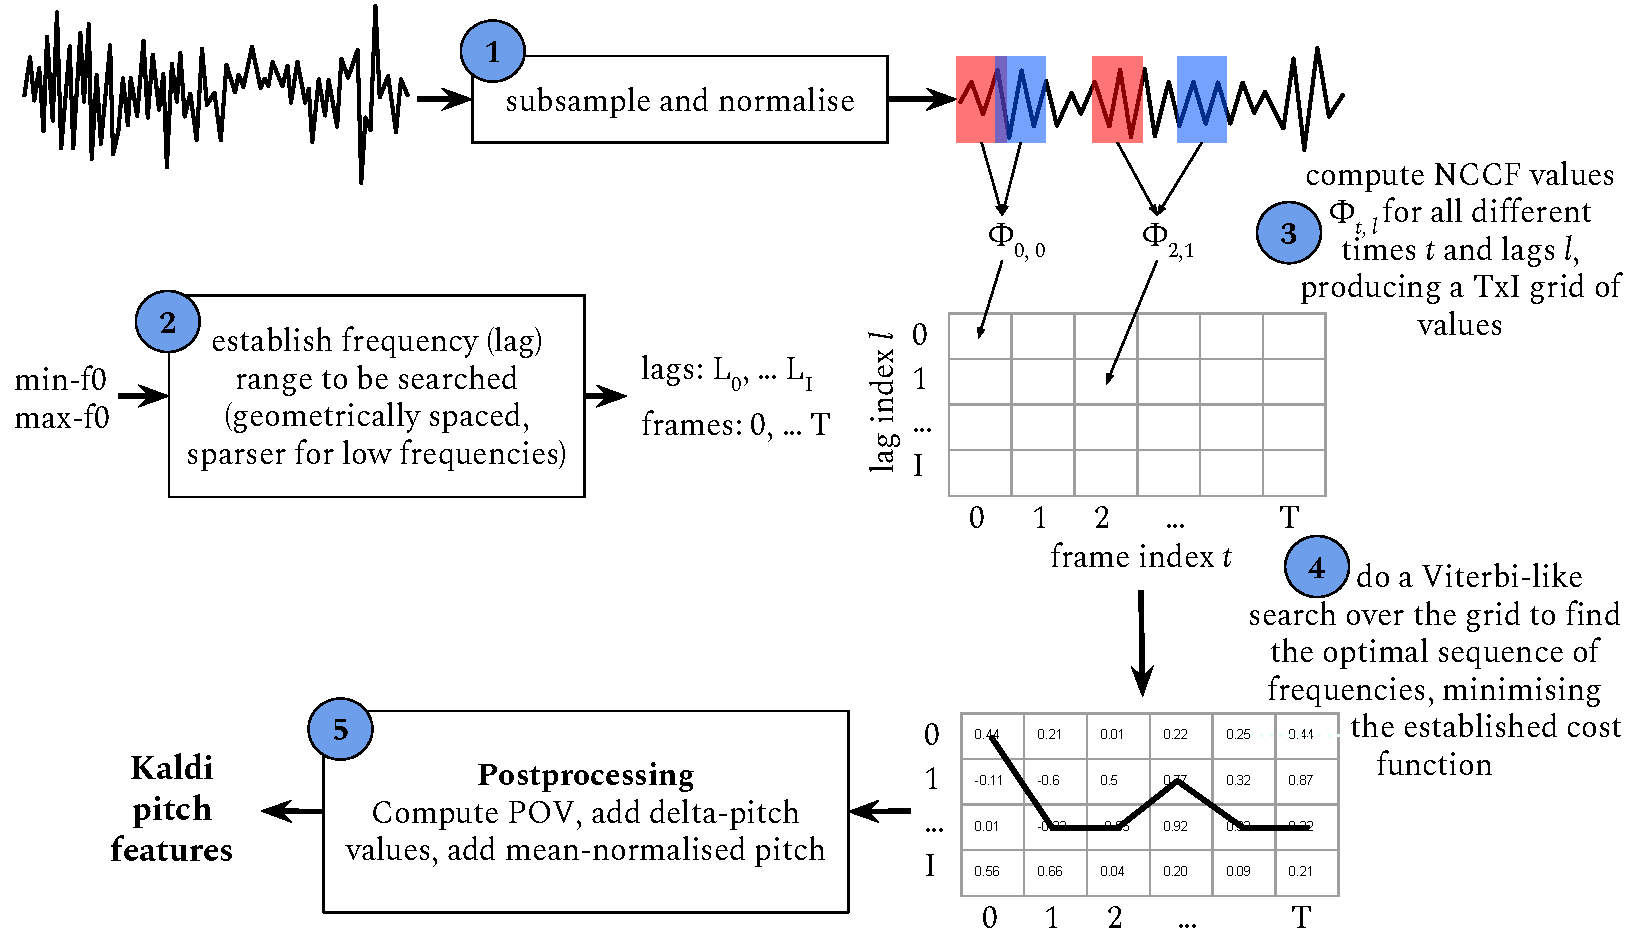
\includegraphics[width=\textwidth]{graphics/kaldi-pitch}
        \vspace*{-1em}
        \caption{The steps of the Kaldi pitch algorithm.}
        \label{fig:kaldi-pitch}
      \end{figure}
      % TO-DO: diagram and formulae describing KaldiPitch.
      % - subsample and normalise (divide by root mean square)
      % - establish frequency range to be searched (geometrically spaced, more sparse for lower frequencies)
      % - compute NCCF for all different time positions and lags, producing a grid of values TxI. the NCCF computation includes the ballast term which makes the values close to zero for very weak normalised cross-correlation values
      % - define cost function for a sequence of frequencies (a pitch contour): penalising low NCCF values, too low frequencies and big frequency jumps
      % - do a Viterbi-based search over the grid to find the optimal sequence of frequencies
      % Postprocessing:
      % on top of the raw pitch, add:
      % - probability of voicing (POV): converting the NCCF values (which have range [-1,1]) to a feature which was empirically found to work well for ASR in multiple languages
      % - normalised pitch: weighted-mean subtraction over windows of 151 frames (+-75), with weights roughly corresponding to log(p(voiced)/p(unvoiced))
      % - delta terms computed over windows of +- 2 frames from the unnormalised pitch
      Perhaps the biggest contribution lies in abandoning the binary decision making about voiced/unvoiced speech, and only calculating pitch for the voiced frames. Instead, soft decisions are made based on the values of the normalised cross-correlation function (NCCF). For two pieces of digitised waveform separated by temporal distance $l$ from each other and represented as vectors $\mathbf{v}_{t, 0}$ and $\mathbf{v}_{t, l}$, the NCCF is computed as follows (adapted from \citeauthor[Eq. 2]{Ghahremani_et_al_2014}):
      \begin{equation}
        \label{eq:nccf}
        \Phi_{t, l} = \frac{\mathbf{v}_{t, 0}^T \mathbf{v}_{t, l}}{\sqrt{(\mathbf{v}_{t, 0}^T \mathbf{v}_{t, 0})(\mathbf{v}_{t, l}^T \mathbf{v}_{t, l})+B}}
      \end{equation}
      where normally $B=0$, but the authors use a non-zero value to push the NCCF values towards 0 where the cross-correlation on its own is very low. By computing NCCF for different spacings $l$  -- called \textit{lags} by the authors, and being effectively the periods of different hypothesised frequencies -- one obtains continuous confidence values about the presence of the corresponding frequencies in the signal for the time position $t$. After computing these for all temporal positions, the algorithm finds the optimal continuous contour by minimising the proposed cost function (see \citeauthor[Eq. 4]{Ghahremani_et_al_2014}), which prefers higher NCCF values and penalises too low frequencies and too big frequency jumps.

      Finally, the algorithm post-processes the raw pitch contour to provide these additional features:
      \begin{enumerate}
        \item {A mean-normalised pitch contour, with the mean computed over 151-frame windows and weighted by a measure roughly corresponding to the log likelihood of a particular frame being voiced (i.e. putting more weight on voiced frames).}
        \item {\textit{Probability of voicing} (POV): A feature which is not a probability, but acts similarly and has been empirically found by the authors to provide improvements in ASR performance.}
        \item {Delta-pitch terms, computed in the same way as the simple deltas in \autoref{eq:dynamic-feats}.}
      \end{enumerate}
    }

    \subsection{Illustrating the prosodic features used in this work}{
      \begin{figure}[h!]
        \centering
        \hspace*{-2.5cm}
        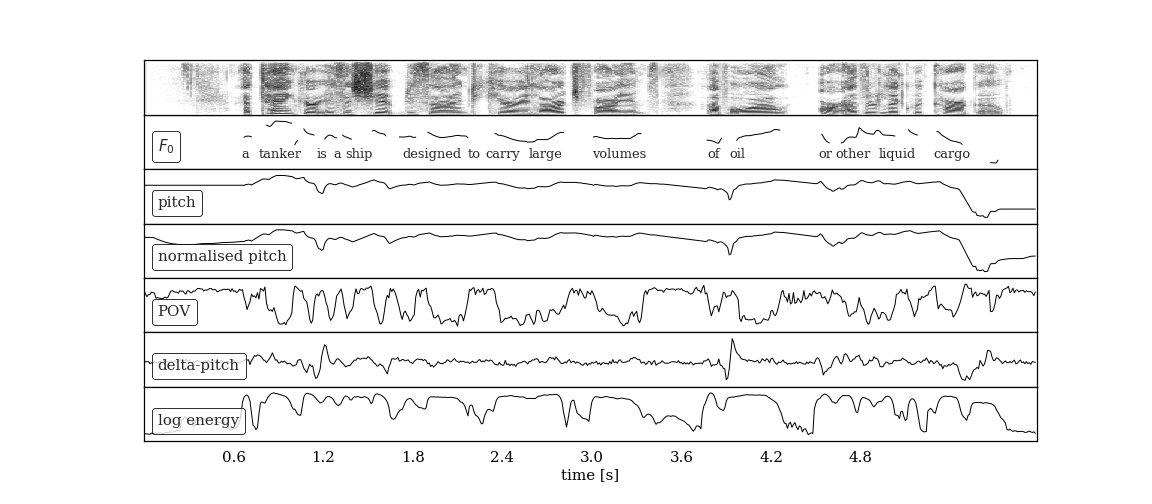
\includegraphics[width=19cm]{../img/prosody_sample}
        \vspace*{-3em}
        \caption{The steps of the Kaldi pitch algorithm.}
        \label{fig:kaldi-pitch}
      \end{figure}
    }
  }
}

\chapter{Data}{
  Intro: Historically, speech corpora were meant for ASR, but now used for LID and SID as well. Since 1996, NIST has also been organising Language Recognition Challenges (LREs), and the corpora used for LREs are now the typically used ones when it comes to evaluating different systems. However, NIST traditionally focuses on telephone, narrowband (8kHz) speech, which represents only one part of all the possible settings in which LID or SID are deployed. In this work, I use a relatively small (< 40GB) corpus which, however, has many qualities that the various NIST corpora lack.

  \section{GlobalPhone}{
    Presented by \cite{Schultz_et_al_2013}, originally for ASR. Wideband (16kHz), recorded native speakers of 23 languages reading newspaper articles -- very similar to the English corpora such as CSR-I, which are based on Wall Street Journal articles. Unlike in NIST corpora, the recording equipment and conditions vary very little. One disadvantage of GlobalPhone is the lack of spontaneous speech. On the other hand, the language goes well beyond the simple conversational language found in the NIST telephone speech corpora.
  }

  \section{Data partitioning}{
    GlobalPhone comes with a partitioning of each language's data into training, development and evaluation datasets, with the sizes of the datasets being roughly 80\%, 10\%, 10\%, respectively. However, for the purposes of the x-vector architecture, 4-way partitioning is required:
    \begin{enumerate}
      \item{training set -- for training the x-vector TDNN,}
      \item{enrollment set -- for training the x-vector classifier,}
      \item{evaluation set ('development' in the GlobalPhone terminology) -- for tuning the hyperparameters of both the TDNN and the classifier,}
      \item{testing set -- for final performance evaluation on unseen data.}
    \end{enumerate}

    In order to use GlobalPhone with the x-vector system, I allocated part of the training data for enrollment. I tried to preserve the GlobalPhone development sets and evaluation sets (which I refer to as evaluation and testing sets, respectively), in order to enable fair comparison of my results obtained on those data portions with any other works that use the GlobalPhone corpus.

    Taking into account the relatively small number of parameters of the x-vector classifier when compared to the x-vector TDNN, I split the training data such that approximately only one 8th is used for enrollment. This way, the training data accounts for roughly 70\% of the whole corpus, while the 3 other portions are roughly 10\% each.

    Importantly, GlobalPhone (as of the GlobalPhone Documentation v4.1) still misses the partitioning for certain languages:
    \begin{enumerate}
      \item {no partitioning for Czech, Polish, Tamil, Swahili, Ukrainian, Vietnamese and Shanghai Chinese,}
      \item {only partial partitioning for Arabic, French, Japanese, Russian.}
    \end{enumerate}

    The {\texttt GlobalPhone} Kaldi recipe contains an extended partitioning, which fixes Czech, French, Japanese, Polish, Russian, Swahili and Vietnamese. For the rest of the languages with incomplete partitioning (Arabic, Tamil, Ukrainian and Shanghai Chinese), I created the partitioning myself, following the same approach as the GlobalPhone authors: "No speaker appears in more than one group and no article was read by two speakers from different groups" (TO-DO: reference the GP docs).

    Some languages didn't have speaker-article data; for those, the partitioning was done randomly.

    For some languages, I could not construct a partitioning with zero article overlap; for those, I tried to at least minimise the overlap.    
  }

  \section{Initial data preprocessing}{
    Basically, SHN to WAV

    Splitting long utterances into shorter ones uniformly, to be able to do classifier training and end-to-end evaluation on segments of different lengths -- like in \cite{Snyder_et_al_2018}. One future improvement would be to not do uniform splitting, but rather split on breaks -- to prevent potentially bad edge effects.
  }

  \section{Invalid data}{
    This was discovered while preprocessing the data from .shn to .wav:
    \begin{enumerate}
      \item {Hausa, Swahili and Ukrainian have broken data.}
      \item {Bulgarian, German, Russian, Turkish and Vietnamese have one broken utterance recording each -- not a big deal, as the number of utterances per language is in hundreds.}
      \item {Portuguese has 2 speakers with almost all data broken (these were discarded), and other 10 speakers with up to 3 broken utterance recordings each (these were keps)}
    \end{enumerate}

    This leaves us with 19 languages, which are used further in this work: Arabic (AR), Bulgarian (BG), Mandarin Chinese (CH), Croatian (CR), Czech (CZ), French (FR), German (GE), Japanese (JA), Korean (KO), Polish (PL), Portuguese (PO), Russian (RU), Spanish (SP), Swedish (SW), Tamil (TA), Thai (TH), Turkish (TU), Vietnamese (VN) and Shanghai Chinese (WU).
  }
}

\chapter{Implementation}{
  \section{The Kaldi toolkit}{
    System was built in Kaldi \citep{Povey_et_al_2011}. (Introduce Kaldi.)
  }
  \section{Adapted implementations}{
    Describe the SRE16 Kaldi recipe, the GlobalPhone ASR recipe, and how they were combined (also using the information from \cite{Snyder_et_al_2018}) to reproduce the LID x-vector system.
  }

  \section{Choice of classifier}{
    The SRE16 recipe uses PLDA, but for verification, not for classification. For our purposes, we needed a proper classifier. Current popular and well-performing classifiers are various flavours of GMM and logistic regression, with no clear winner. \cite{Snyder_et_al_2018}, for instance, used GMM trained using MMI -- based on \cite{McCree_2014}. I decided to re-use a model which is already implemented in the LRE07/v2 Kaldi recipe -- logistic regression. The decision was also consulted with \cite{Snyder_2018_kaldi-help}. One theoretical downside of logistic regression is that the resulting decision boundaries are linear, whereas with GMM (trained with full co-variance matrix), one can achieve more complex quadratic decision boundaries. On the other hand though, training a full covariance requires much data, and the enrollment set would likely be not big enough. Additionally, the Kaldi logit can describe each class using more than linear boundary (see next section), so the decision boundaries should be complex enough to be able to model the observed data well.
  }

  \section{Final architecture}{
    Description of x-vector+GP architecture (highlighting own contributions)

    how the whole pipeline works: go into much more detail than in the Related work section

    description of the Kaldi logit, which models each class using multiple "mixtures", i.e. multiple boundaries
    
    mention possibility of direct classification with TDNN and that I focus on using separate classifier because it provides extra flexibility and because it was shown to perform slightly better
  }

  \section{Computing environment}{
    cluster, Slurm, GPUs, parallelisation, rough runtimes of the different stages (TDNN training, x-vector extraction, logit training, inference)
  }

  \section{Hyperparameters}{
    decided: TDNN layers, activation function, learning algorithm (TO-DO: read about shrinking)

    tuned (using the baseline setting, see next chapter): number of TDNN training epochs, logit hyperparameters
  }
}

\chapter{Experiments}{
  Intro: I will compare a selection of acoustic and prosodic features. Despite their reported potential, I don't use BNFs in this work, as they are basically just a higher-level feature based on the acoustic MFCC information (at least the BNFs in \cite{Snyder_et_al_2018}).

  Evaluation metric: $C_{primary}$, consistent with NIST LREs. Elaborate a bit more on the meaning of the metric, maybe compare with accuracy and other simpler metrics.

  \section{Baseline}{
    vanilla MFCCs (no deltas): also comment on the decisions made regarding MFCC MFCC configuration

    $\leq 30s$ enrollment segments, $\leq 10s$ eval/test segments (should be possible to also report exact average segment length for each set)
  }

  \section{Shifted delta cepstra}{
    Want to see whether context aggregation in the form of added deltas in SDCs (compared to vanilla MFCCs) can improve performance, since the TDNN does context aggregation of its own.
  }

  \section{KaldiPitch+Energy vectors}{
    Calculating pitch even for unvoiced frames using the algorithm presented by \cite{Ghahremani_et_al_2014}. Adding raw energy to model stress. Extremely low-dimensionality feature vectors, but will see how the TDNN and classifier trained on these can do prosodic LID. Hoping to achieve some sensible results, probably much worse than with MFCCs or SDCs.
  }
  
  \section{MFCC/SDC + KaldiPitch+Energy}{
    Taking the winner from MFCC/SDC, and concatenating those features with Kaldi pitch and raw energy values. Training the TDNN and classifier on that. Hopefully, seeing an improvement.
  }
  
  \section{Fusion of MFCC/SDC and KaldiPitch+Energy scores}{
    Stretch goal, likely to be delayed for Year 5 (or abandoned if there are more attractive ideas)

    Same as previous section, but scores computed separately (using two systems, one trained on acoustic features, the other one on prosodic) and fused using a logit fuser. Probably using evaluation set for training the fuser (although, ideally, a separate data portion would be reserved for that).
  }

  \section{Timeline for the experiments}{
    \label{timeline}
    \begin{enumerate}
      \item {
        Finished: System using MFCC and SDC.
      }
      \item {
        By January 28th: Choose the TDNN and logit hyperparameters. TDNN using MFCCs has already been trained for, 2, 3, ... 10 epochs, now need to 1) establish reasonable logit parameters (driven by evaluation-set performance on x-vectors from TDNN trained for 3 epochs), 2) use that logit config to score the TDNNs with different number of training epochs, 3) choose a number of epochs that is a reasonable compromise between performance and training runtime
      }
      \item {
        By February 4th: Have MFCC vs SDC comparison carried out (includes baseline results using MFCCs). Have KaldiPitch and raw energy features implemented (both are straightforward to compute with Kaldi -- the energy is just computing MFCCs with raw log energy instead of C0, and discarding all but the energy-corresponding resulting coefficient). Have splicing of MFCC/SDC features with prosodic features implemented.
      }
      \item {
        By February 11th: Have results of KaldiPitch+Energy experiments and of the acoustic+prosodic experiment (MFCC/SDC + KaldiPitch+Energy)
      }
    \end{enumerate}
  }
}

\chapter{Results}{
  Reporting: overall $C_{primary}$, accuracy (for illustrative purposes), confusion matrix (to see which language pairs are confusing)
  
  Focus on Slavic languages, since there is so many of them (Czech, Croatian, Polish, Russian, Bulgarian) and intonation can be very characteristic and important here (my own intuition, based on my knowledge of Slavic languages).
}

\chapter{Discussion}{
  
}

\chapter{Future work}{
  \section{Plans for Part 2 of the MInf project}{

  }

  \section{Other future ideas}{
    Everything that is sensible but unlikely in Year 5.
  }
}

\chapter{Conclusions}{
  
}

% TO-DO: Make sure 'Proc.' is where it has to be (some entries are marked as @article when they should be @inproceedings)
\bibliographystyle{apalike}
\bibliography{s1513472-minf1}

\end{document}
